%%%%%%%%%%%%%%%%%%%%%%%%%%%%%%%%%%%%%%%%%
% University Assignment Title Page 
% LaTeX Template
% Version 1.0 (27/12/12)
%
% This template has been downloaded from:
% http://www.LaTeXTemplates.com
%
% Original author:
% WikiBooks (http://en.wikibooks.org/wiki/LaTeX/Title_Creation)
%
% License:
% CC BY-NC-SA 3.0 (http://creativecommons.org/licenses/by-nc-sa/3.0/)
% 
% Instructions for using this template:
% This title page is capable of being compiled as is. This is not useful for 
% including it in another document. To do this, you have two options: 
%
% 1) Copy/paste everything between \begin{document} and \end{document} 
% starting at \begin{titlepage} and paste this into another LaTeX file where you 
% want your title page.
% OR
% 2) Remove everything outside the \begin{titlepage} and \end{titlepage} and 
% move this file to the same directory as the LaTeX file you wish to add it to. 
% Then add %%%%%%%%%%%%%%%%%%%%%%%%%%%%%%%%%%%%%%%%%
% University Assignment Title Page 
% LaTeX Template
% Version 1.0 (27/12/12)
%
% This template has been downloaded from:
% http://www.LaTeXTemplates.com
%
% Original author:
% WikiBooks (http://en.wikibooks.org/wiki/LaTeX/Title_Creation)
%
% License:
% CC BY-NC-SA 3.0 (http://creativecommons.org/licenses/by-nc-sa/3.0/)
% 
% Instructions for using this template:
% This title page is capable of being compiled as is. This is not useful for 
% including it in another document. To do this, you have two options: 
%
% 1) Copy/paste everything between \begin{document} and \end{document} 
% starting at \begin{titlepage} and paste this into another LaTeX file where you 
% want your title page.
% OR
% 2) Remove everything outside the \begin{titlepage} and \end{titlepage} and 
% move this file to the same directory as the LaTeX file you wish to add it to. 
% Then add %%%%%%%%%%%%%%%%%%%%%%%%%%%%%%%%%%%%%%%%%
% University Assignment Title Page 
% LaTeX Template
% Version 1.0 (27/12/12)
%
% This template has been downloaded from:
% http://www.LaTeXTemplates.com
%
% Original author:
% WikiBooks (http://en.wikibooks.org/wiki/LaTeX/Title_Creation)
%
% License:
% CC BY-NC-SA 3.0 (http://creativecommons.org/licenses/by-nc-sa/3.0/)
% 
% Instructions for using this template:
% This title page is capable of being compiled as is. This is not useful for 
% including it in another document. To do this, you have two options: 
%
% 1) Copy/paste everything between \begin{document} and \end{document} 
% starting at \begin{titlepage} and paste this into another LaTeX file where you 
% want your title page.
% OR
% 2) Remove everything outside the \begin{titlepage} and \end{titlepage} and 
% move this file to the same directory as the LaTeX file you wish to add it to. 
% Then add %%%%%%%%%%%%%%%%%%%%%%%%%%%%%%%%%%%%%%%%%
% University Assignment Title Page 
% LaTeX Template
% Version 1.0 (27/12/12)
%
% This template has been downloaded from:
% http://www.LaTeXTemplates.com
%
% Original author:
% WikiBooks (http://en.wikibooks.org/wiki/LaTeX/Title_Creation)
%
% License:
% CC BY-NC-SA 3.0 (http://creativecommons.org/licenses/by-nc-sa/3.0/)
% 
% Instructions for using this template:
% This title page is capable of being compiled as is. This is not useful for 
% including it in another document. To do this, you have two options: 
%
% 1) Copy/paste everything between \begin{document} and \end{document} 
% starting at \begin{titlepage} and paste this into another LaTeX file where you 
% want your title page.
% OR
% 2) Remove everything outside the \begin{titlepage} and \end{titlepage} and 
% move this file to the same directory as the LaTeX file you wish to add it to. 
% Then add \input{./title_page_1.tex} to your LaTeX file where you want your
% title page.
%
%%%%%%%%%%%%%%%%%%%%%%%%%%%%%%%%%%%%%%%%%
%\title{Title page with logo}
%----------------------------------------------------------------------------------------
%	PACKAGES AND OTHER DOCUMENT CONFIGURATIONS
%----------------------------------------------------------------------------------------

\documentclass[12pt]{article}
\usepackage[english]{babel}
\usepackage[utf8x]{inputenc}
\usepackage{amsmath}
\usepackage{graphicx}
\usepackage{algorithm}
\usepackage[noend]{algpseudocode}
\usepackage[colorinlistoftodos]{todonotes}

\begin{document}

\begin{titlepage}

\newcommand{\HRule}{\rule{\linewidth}{0.5mm}} % Defines a new command for the horizontal lines, change thickness here

\center % Center everything on the page
 
%----------------------------------------------------------------------------------------
%	HEADING SECTIONS
%----------------------------------------------------------------------------------------

\textsc{\LARGE University of Texas at San Antonio}\\[1.5cm] % Name of your university/college
\textsc{\Large Department of Computer Science}\\[0.5cm] % Major heading such as course name
\textsc{\large CS-6953-012: Independent Study}\\[0.5cm] % Minor heading such as course title

%----------------------------------------------------------------------------------------
%	TITLE SECTION
%----------------------------------------------------------------------------------------

\HRule \\[0.4cm]
{ \huge \bfseries Feature Selection in TF-DNA using Correlation Analysis}\\[0.4cm] % Title of your document
\HRule \\[1.5cm]
 
%----------------------------------------------------------------------------------------
%	AUTHOR SECTION
%----------------------------------------------------------------------------------------

\begin{minipage}{0.4\textwidth}
\begin{flushleft} \large
\emph{Author:}\\
Rifatul Islam % Your name
\end{flushleft}
\end{minipage}
~
\begin{minipage}{0.4\textwidth}
\begin{flushright} \large
\emph{Supervisor:} \\
Dr. Jianhua Ruan % Supervisor's Name
\end{flushright}
\end{minipage}\\[2cm]

% If you don't want a supervisor, uncomment the two lines below and remove the section above
%\Large \emph{Author:}\\
%John \textsc{Smith}\\[3cm] % Your name

%----------------------------------------------------------------------------------------
%	LOGO SECTION
%----------------------------------------------------------------------------------------


\includegraphics{logo.jpg}\\[1cm] % Include a department/university logo - this will require the graphicx package

%----------------------------------------------------------------------------------------
%	DATE SECTION
%----------------------------------------------------------------------------------------

 {\large \today}\\[2cm] % Date, change the \today to a set date if you want to be precise

%----------------------------------------------------------------------------------------

\vfill % Fill the rest of the page with whitespace

\end{titlepage}

\begin{abstract}
Feature selection of the genes with respect to their corresponding TF is an important study in bioinformatics and generally researchers in bioinformatics want to know which conditions in genes and corresponding TF-DNA are related. In this study we investigated how can we extract the important features from the gene expression that are correlated with the corresponding TF using correlation analysis. We proposed a correlation based algorithm that selects the appropriate gene conditions based on correlation measurement and outputs the gene conditions that are highly related. 

\end{abstract}

\section{Introduction}
The protein that controls the rate of transcription of genetic information from DNA to messenger RNA by binding to a specific DNA sequence is known as the Transcription Factor(TF) which plays an important role in regulating genes \cite{wiki:tf123}. TFs work in coordination with other proteins by activating or blocking the RNA polymerase to specific genes. Transcription factors bind to either enhancer or promoter regions of DNA adjacent to the genes that they regulate. In this paper I tried to investigate which gene conditions are highly correlated with their corresponding TFs. We conduct our study based on simulated TF and Gene expression and used correlation analysis to extract the important feature from the genes. \\

We presented an algorithm that can extract the features from a given TF and their corresponding GENEs. In our study we designed a data generator that can generate the random data for the TF and the corresponding Genes. We intentionally put random data and values that are not correlated. Finally we used our algorithm to extract the correlated conditions from the random set of data. The algorithm works with an average accuracy of 90\%. 
\\ 

In the following section I will be discussing more details about our approach and results. Section 2 will include the Details of our experiments we presented the algorithm in section 2.2. In section 3 we discussed about the future direction of this study and how it can be improved further. We conclude our work by discussion the limitation of our algorithm. 


\section{Methodology}
In this section we will be discussing about the details about our approach to feature selection. To conduct our experiment we generate the TF and Gene data randomly with some data uniform random generation that generates data randomly with some intended not correlated data. Then we shuffle the data enough time so that the correlated and non-correlated data is mixed up. The goal is to figure out those conditions in the GENE data which are correlated with their corresponding Transcription Factor. The following section contains more detailed about the experiment setup, algorithm and result. 

\subsection{Experiment Setup}
We conducted our experiment in a core i7(7th Gen) with 16GB of RAM machine running on Linux based operating system(Ubuntu 18.04). We choose python version:3.6 as a programming language for convenience with the availability of data analysis packages. For data generation we use normal distribution with some intentionally added non-correlated data. For example: with 100 TF data randomly generated we generate 80 corresponding GENE values were generated that are correlated and 20 are generated that are not correlated. We use standard shuffling method to mix the correlated and non-correlated data. Then our algorithm was designed to extract the highest correlated gene value(in this case 80) that are correlated with the corresponding TF value.

\subsection{Algorithm}
In this subsection we will be discussing our algorithm in extracting the important feature of the generated TF and GENE data. Our algorithm is an iterative based algorithm which takes input as the GENE values $G$ and TF value $T$ and returns the list of correlated GENE value $G_{cor}$ and TF value $T_{cor}$. Our algorithm uses Pearson correlation analysis to select the correlated features in an iterative manner.

In this subsection we will be discussing our algorithm in extracting the important feature of the generated TF and GENE data. Our algorithm is an iterative based algorithm which takes input as the GENE values $G$ and TF value $T$ and returns the list of correlated GENE value $G_{cor}$ and TF value $T_{cor}$. Our algorithm uses Pearson correlation analysis to select the correlated features in an iterative manner.

In this subsection we will be discussing our algorithm in extracting the important feature of the generated TF and GENE data. Our algorithm is an iterative based algorithm which takes input as the GENE values $G$ and TF value $T$ and returns the list of correlated GENE value $G_{cor}$ and TF value $T_{cor}$. Our algorithm uses Pearson correlation analysis to select the correlated features in an iterative manner.


\begin{algorithm}
\caption{Iterative Feature Selection}\label{iter}
\begin{algorithmic}[1]
\Procedure{Iter correlation}{T, G, n}

\State $ GN_{corr}, TF_{corr} \gets  \textit{top\_fitted(T, G)}$
\State $ G', T'  \gets  \textit{update(T,G, TF\_{corr}, GN\_{corr})} $

\While {($\forall \, value \,\, G' \, and \, T' $)}: 
	\For {($item \, in \,G' \, and \, T'$)}:
    	\State $ GN_{corr}, TF_{corr} \gets G[item], T[item]$
        \State $corr[] \gets pearsonr(GN_{corr}, TF_{corr})$
    \EndFor
    
    \State bucket $\gets$ \( \log_2 |G'| \)
    \State $ GN_{corr} , TF_{corr} \gets  \textit{choose(T', G', bucket, corr[])}$
   \State $ G', T'  \gets  \textit{update(T,G, TF\_{corr}, GN\_{corr})} $
\EndWhile

\For {($item \,\, in \,GN_{corr} \, and \, TF_{corr}$)}:
    \State $ GN_{corr}, TF_{corr} \gets G[item], T[item]$
    \State $corr[] \gets pearsonr(GN_{corr}, TF_{corr})$
\EndFor

\EndProcedure
\end{algorithmic}
\end{algorithm}

In this subsection we will be discussing our algorithm in extracting the important feature of the generated TF and GENE data. Our algorithm is an iterative based algorithm which takes input as the GENE values $G$ and TF value $T$ and returns the list of correlated GENE value $G_{cor}$ and TF value $T_{cor}$. Our algorithm uses Pearson correlation analysis to select the correlated features in an iterative manner.


\subsection{Result}

Use the table  and tabular commands for basic tables --- see Table~\ref{tab:widgets}, for example. You can upload a figure (JPEG, PNG or PDF) using the files menu. To include it in your document, use the includegraphics command as in the code for Figure~\ref{fig:frog} below.

% Commands to include a figure:
% \begin{figure}
% \centering
% 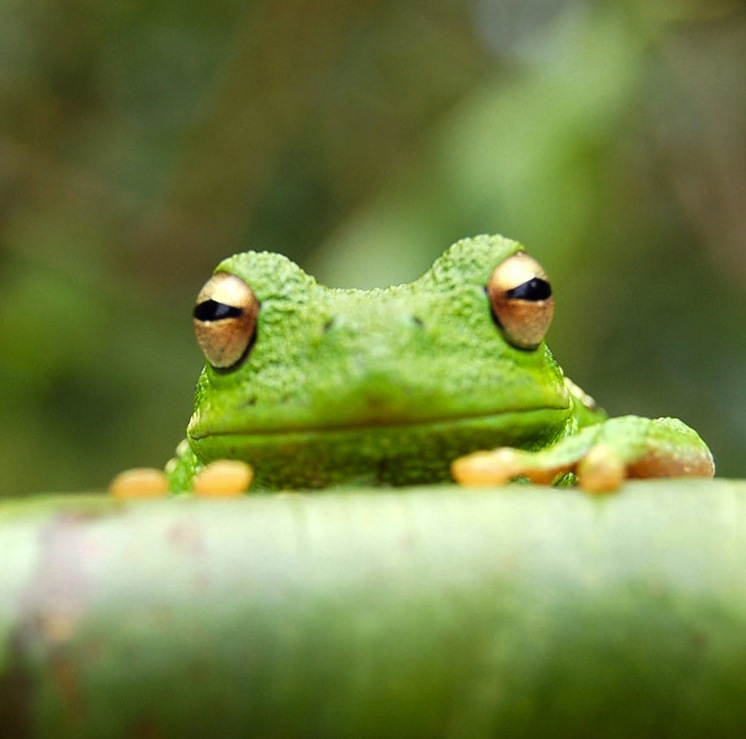
\includegraphics[width=0.5\textwidth]{frog.jpg}
% \caption{\label{fig:frog}This is a figure caption.}
% \end{figure}

% \begin{table}
% \centering
% \begin{tabular}{l|r}
% Item & Quantity \\\hline
% Widgets & 42 \\
% Gadgets & 13
% \end{tabular}
% \caption{\label{tab:widgets}An example table.}
% \end{table}

\section{Future Works}

\LaTeX{} is great at typesetting mathematics. Let $X_1, X_2, \ldots, X_n$ be a sequence of independent and identically distributed random variables with $\text{E}[X_i] = \mu$ and $\text{Var}[X_i] = \sigma^2 < \infty$, and let
$$S_n = \frac{X_1 + X_2 + \cdots + X_n}{n}
      = \frac{1}{n}\sum_{i}^{n} X_i$$
denote their mean. Then as $n$ approaches infinity, the random variables $\sqrt{n}(S_n - \mu)$ converge in distribution to a normal $\mathcal{N}(0, \sigma^2)$.

\section{Conclusion}

You can make lists with automatic numbering \dots

\begin{enumerate}
\item Like this,
\item and like this.
\end{enumerate}
\dots or bullet points \dots
\begin{itemize}
\item Like this,
\item and like this.
\end{itemize}

We hope you find write\LaTeX\ useful, and please let us know if you have any feedback using the help menu above.

\bibliographystyle{acm}
\bibliography{bib1.bib}

\end{document} to your LaTeX file where you want your
% title page.
%
%%%%%%%%%%%%%%%%%%%%%%%%%%%%%%%%%%%%%%%%%
%\title{Title page with logo}
%----------------------------------------------------------------------------------------
%	PACKAGES AND OTHER DOCUMENT CONFIGURATIONS
%----------------------------------------------------------------------------------------

\documentclass[12pt]{article}
\usepackage[english]{babel}
\usepackage[utf8x]{inputenc}
\usepackage{amsmath}
\usepackage{graphicx}
\usepackage{algorithm}
\usepackage[noend]{algpseudocode}
\usepackage[colorinlistoftodos]{todonotes}

\begin{document}

\begin{titlepage}

\newcommand{\HRule}{\rule{\linewidth}{0.5mm}} % Defines a new command for the horizontal lines, change thickness here

\center % Center everything on the page
 
%----------------------------------------------------------------------------------------
%	HEADING SECTIONS
%----------------------------------------------------------------------------------------

\textsc{\LARGE University of Texas at San Antonio}\\[1.5cm] % Name of your university/college
\textsc{\Large Department of Computer Science}\\[0.5cm] % Major heading such as course name
\textsc{\large CS-6953-012: Independent Study}\\[0.5cm] % Minor heading such as course title

%----------------------------------------------------------------------------------------
%	TITLE SECTION
%----------------------------------------------------------------------------------------

\HRule \\[0.4cm]
{ \huge \bfseries Feature Selection in TF-DNA using Correlation Analysis}\\[0.4cm] % Title of your document
\HRule \\[1.5cm]
 
%----------------------------------------------------------------------------------------
%	AUTHOR SECTION
%----------------------------------------------------------------------------------------

\begin{minipage}{0.4\textwidth}
\begin{flushleft} \large
\emph{Author:}\\
Rifatul Islam % Your name
\end{flushleft}
\end{minipage}
~
\begin{minipage}{0.4\textwidth}
\begin{flushright} \large
\emph{Supervisor:} \\
Dr. Jianhua Ruan % Supervisor's Name
\end{flushright}
\end{minipage}\\[2cm]

% If you don't want a supervisor, uncomment the two lines below and remove the section above
%\Large \emph{Author:}\\
%John \textsc{Smith}\\[3cm] % Your name

%----------------------------------------------------------------------------------------
%	LOGO SECTION
%----------------------------------------------------------------------------------------


\includegraphics{logo.jpg}\\[1cm] % Include a department/university logo - this will require the graphicx package

%----------------------------------------------------------------------------------------
%	DATE SECTION
%----------------------------------------------------------------------------------------

 {\large \today}\\[2cm] % Date, change the \today to a set date if you want to be precise

%----------------------------------------------------------------------------------------

\vfill % Fill the rest of the page with whitespace

\end{titlepage}

\begin{abstract}
Feature selection of the genes with respect to their corresponding TF is an important study in bioinformatics and generally researchers in bioinformatics want to know which conditions in genes and corresponding TF-DNA are related. In this study we investigated how can we extract the important features from the gene expression that are correlated with the corresponding TF using correlation analysis. We proposed a correlation based algorithm that selects the appropriate gene conditions based on correlation measurement and outputs the gene conditions that are highly related. 

\end{abstract}

\section{Introduction}
The protein that controls the rate of transcription of genetic information from DNA to messenger RNA by binding to a specific DNA sequence is known as the Transcription Factor(TF) which plays an important role in regulating genes \cite{wiki:tf123}. TFs work in coordination with other proteins by activating or blocking the RNA polymerase to specific genes. Transcription factors bind to either enhancer or promoter regions of DNA adjacent to the genes that they regulate. In this paper I tried to investigate which gene conditions are highly correlated with their corresponding TFs. We conduct our study based on simulated TF and Gene expression and used correlation analysis to extract the important feature from the genes. \\

We presented an algorithm that can extract the features from a given TF and their corresponding GENEs. In our study we designed a data generator that can generate the random data for the TF and the corresponding Genes. We intentionally put random data and values that are not correlated. Finally we used our algorithm to extract the correlated conditions from the random set of data. The algorithm works with an average accuracy of 90\%. 
\\ 

In the following section I will be discussing more details about our approach and results. Section 2 will include the Details of our experiments we presented the algorithm in section 2.2. In section 3 we discussed about the future direction of this study and how it can be improved further. We conclude our work by discussion the limitation of our algorithm. 


\section{Methodology}
In this section we will be discussing about the details about our approach to feature selection. To conduct our experiment we generate the TF and Gene data randomly with some data uniform random generation that generates data randomly with some intended not correlated data. Then we shuffle the data enough time so that the correlated and non-correlated data is mixed up. The goal is to figure out those conditions in the GENE data which are correlated with their corresponding Transcription Factor. The following section contains more detailed about the experiment setup, algorithm and result. 

\subsection{Experiment Setup}
We conducted our experiment in a core i7(7th Gen) with 16GB of RAM machine running on Linux based operating system(Ubuntu 18.04). We choose python version:3.6 as a programming language for convenience with the availability of data analysis packages. For data generation we use normal distribution with some intentionally added non-correlated data. For example: with 100 TF data randomly generated we generate 80 corresponding GENE values were generated that are correlated and 20 are generated that are not correlated. We use standard shuffling method to mix the correlated and non-correlated data. Then our algorithm was designed to extract the highest correlated gene value(in this case 80) that are correlated with the corresponding TF value.

\subsection{Algorithm}
In this subsection we will be discussing our algorithm in extracting the important feature of the generated TF and GENE data. Our algorithm is an iterative based algorithm which takes input as the GENE values $G$ and TF value $T$ and returns the list of correlated GENE value $G_{cor}$ and TF value $T_{cor}$. Our algorithm uses Pearson correlation analysis to select the correlated features in an iterative manner.

In this subsection we will be discussing our algorithm in extracting the important feature of the generated TF and GENE data. Our algorithm is an iterative based algorithm which takes input as the GENE values $G$ and TF value $T$ and returns the list of correlated GENE value $G_{cor}$ and TF value $T_{cor}$. Our algorithm uses Pearson correlation analysis to select the correlated features in an iterative manner.

In this subsection we will be discussing our algorithm in extracting the important feature of the generated TF and GENE data. Our algorithm is an iterative based algorithm which takes input as the GENE values $G$ and TF value $T$ and returns the list of correlated GENE value $G_{cor}$ and TF value $T_{cor}$. Our algorithm uses Pearson correlation analysis to select the correlated features in an iterative manner.


\begin{algorithm}
\caption{Iterative Feature Selection}\label{iter}
\begin{algorithmic}[1]
\Procedure{Iter correlation}{T, G, n}

\State $ GN_{corr}, TF_{corr} \gets  \textit{top\_fitted(T, G)}$
\State $ G', T'  \gets  \textit{update(T,G, TF\_{corr}, GN\_{corr})} $

\While {($\forall \, value \,\, G' \, and \, T' $)}: 
	\For {($item \, in \,G' \, and \, T'$)}:
    	\State $ GN_{corr}, TF_{corr} \gets G[item], T[item]$
        \State $corr[] \gets pearsonr(GN_{corr}, TF_{corr})$
    \EndFor
    
    \State bucket $\gets$ \( \log_2 |G'| \)
    \State $ GN_{corr} , TF_{corr} \gets  \textit{choose(T', G', bucket, corr[])}$
   \State $ G', T'  \gets  \textit{update(T,G, TF\_{corr}, GN\_{corr})} $
\EndWhile

\For {($item \,\, in \,GN_{corr} \, and \, TF_{corr}$)}:
    \State $ GN_{corr}, TF_{corr} \gets G[item], T[item]$
    \State $corr[] \gets pearsonr(GN_{corr}, TF_{corr})$
\EndFor

\EndProcedure
\end{algorithmic}
\end{algorithm}

In this subsection we will be discussing our algorithm in extracting the important feature of the generated TF and GENE data. Our algorithm is an iterative based algorithm which takes input as the GENE values $G$ and TF value $T$ and returns the list of correlated GENE value $G_{cor}$ and TF value $T_{cor}$. Our algorithm uses Pearson correlation analysis to select the correlated features in an iterative manner.


\subsection{Result}

Use the table  and tabular commands for basic tables --- see Table~\ref{tab:widgets}, for example. You can upload a figure (JPEG, PNG or PDF) using the files menu. To include it in your document, use the includegraphics command as in the code for Figure~\ref{fig:frog} below.

% Commands to include a figure:
% \begin{figure}
% \centering
% 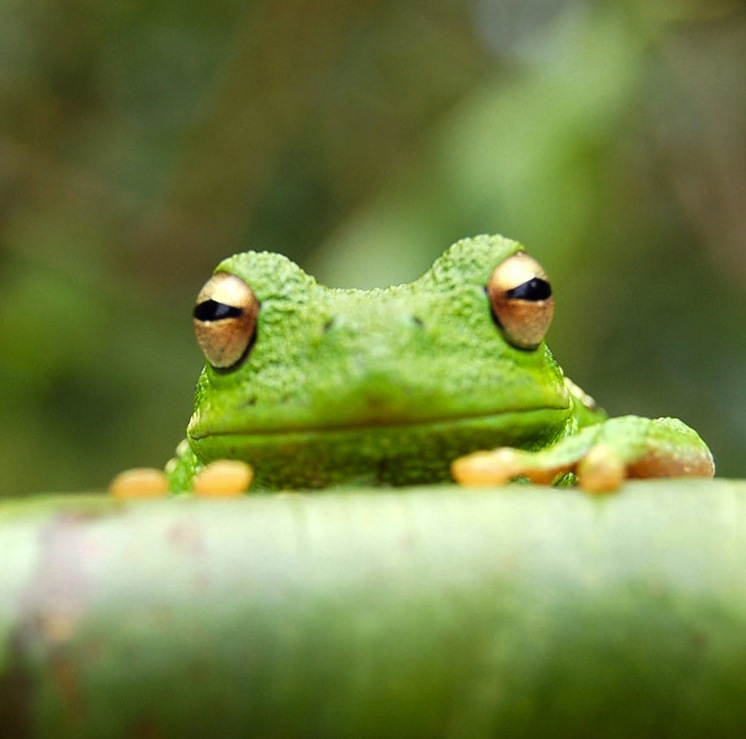
\includegraphics[width=0.5\textwidth]{frog.jpg}
% \caption{\label{fig:frog}This is a figure caption.}
% \end{figure}

% \begin{table}
% \centering
% \begin{tabular}{l|r}
% Item & Quantity \\\hline
% Widgets & 42 \\
% Gadgets & 13
% \end{tabular}
% \caption{\label{tab:widgets}An example table.}
% \end{table}

\section{Future Works}

\LaTeX{} is great at typesetting mathematics. Let $X_1, X_2, \ldots, X_n$ be a sequence of independent and identically distributed random variables with $\text{E}[X_i] = \mu$ and $\text{Var}[X_i] = \sigma^2 < \infty$, and let
$$S_n = \frac{X_1 + X_2 + \cdots + X_n}{n}
      = \frac{1}{n}\sum_{i}^{n} X_i$$
denote their mean. Then as $n$ approaches infinity, the random variables $\sqrt{n}(S_n - \mu)$ converge in distribution to a normal $\mathcal{N}(0, \sigma^2)$.

\section{Conclusion}

You can make lists with automatic numbering \dots

\begin{enumerate}
\item Like this,
\item and like this.
\end{enumerate}
\dots or bullet points \dots
\begin{itemize}
\item Like this,
\item and like this.
\end{itemize}

We hope you find write\LaTeX\ useful, and please let us know if you have any feedback using the help menu above.

\bibliographystyle{acm}
\bibliography{bib1.bib}

\end{document} to your LaTeX file where you want your
% title page.
%
%%%%%%%%%%%%%%%%%%%%%%%%%%%%%%%%%%%%%%%%%
%\title{Title page with logo}
%----------------------------------------------------------------------------------------
%	PACKAGES AND OTHER DOCUMENT CONFIGURATIONS
%----------------------------------------------------------------------------------------

\documentclass[12pt]{article}
\usepackage[english]{babel}
\usepackage[utf8x]{inputenc}
\usepackage{amsmath}
\usepackage{graphicx}
\usepackage{algorithm}
\usepackage[noend]{algpseudocode}
\usepackage[colorinlistoftodos]{todonotes}

\begin{document}

\begin{titlepage}

\newcommand{\HRule}{\rule{\linewidth}{0.5mm}} % Defines a new command for the horizontal lines, change thickness here

\center % Center everything on the page
 
%----------------------------------------------------------------------------------------
%	HEADING SECTIONS
%----------------------------------------------------------------------------------------

\textsc{\LARGE University of Texas at San Antonio}\\[1.5cm] % Name of your university/college
\textsc{\Large Department of Computer Science}\\[0.5cm] % Major heading such as course name
\textsc{\large CS-6953-012: Independent Study}\\[0.5cm] % Minor heading such as course title

%----------------------------------------------------------------------------------------
%	TITLE SECTION
%----------------------------------------------------------------------------------------

\HRule \\[0.4cm]
{ \huge \bfseries Feature Selection in TF-DNA using Correlation Analysis}\\[0.4cm] % Title of your document
\HRule \\[1.5cm]
 
%----------------------------------------------------------------------------------------
%	AUTHOR SECTION
%----------------------------------------------------------------------------------------

\begin{minipage}{0.4\textwidth}
\begin{flushleft} \large
\emph{Author:}\\
Rifatul Islam % Your name
\end{flushleft}
\end{minipage}
~
\begin{minipage}{0.4\textwidth}
\begin{flushright} \large
\emph{Supervisor:} \\
Dr. Jianhua Ruan % Supervisor's Name
\end{flushright}
\end{minipage}\\[2cm]

% If you don't want a supervisor, uncomment the two lines below and remove the section above
%\Large \emph{Author:}\\
%John \textsc{Smith}\\[3cm] % Your name

%----------------------------------------------------------------------------------------
%	LOGO SECTION
%----------------------------------------------------------------------------------------


\includegraphics{logo.jpg}\\[1cm] % Include a department/university logo - this will require the graphicx package

%----------------------------------------------------------------------------------------
%	DATE SECTION
%----------------------------------------------------------------------------------------

 {\large \today}\\[2cm] % Date, change the \today to a set date if you want to be precise

%----------------------------------------------------------------------------------------

\vfill % Fill the rest of the page with whitespace

\end{titlepage}

\begin{abstract}
Feature selection of the genes with respect to their corresponding TF is an important study in bioinformatics and generally researchers in bioinformatics want to know which conditions in genes and corresponding TF-DNA are related. In this study we investigated how can we extract the important features from the gene expression that are correlated with the corresponding TF using correlation analysis. We proposed a correlation based algorithm that selects the appropriate gene conditions based on correlation measurement and outputs the gene conditions that are highly related. 

\end{abstract}

\section{Introduction}
The protein that controls the rate of transcription of genetic information from DNA to messenger RNA by binding to a specific DNA sequence is known as the Transcription Factor(TF) which plays an important role in regulating genes \cite{wiki:tf123}. TFs work in coordination with other proteins by activating or blocking the RNA polymerase to specific genes. Transcription factors bind to either enhancer or promoter regions of DNA adjacent to the genes that they regulate. In this paper I tried to investigate which gene conditions are highly correlated with their corresponding TFs. We conduct our study based on simulated TF and Gene expression and used correlation analysis to extract the important feature from the genes. \\

We presented an algorithm that can extract the features from a given TF and their corresponding GENEs. In our study we designed a data generator that can generate the random data for the TF and the corresponding Genes. We intentionally put random data and values that are not correlated. Finally we used our algorithm to extract the correlated conditions from the random set of data. The algorithm works with an average accuracy of 90\%. 
\\ 

In the following section I will be discussing more details about our approach and results. Section 2 will include the Details of our experiments we presented the algorithm in section 2.2. In section 3 we discussed about the future direction of this study and how it can be improved further. We conclude our work by discussion the limitation of our algorithm. 


\section{Methodology}
In this section we will be discussing about the details about our approach to feature selection. To conduct our experiment we generate the TF and Gene data randomly with some data uniform random generation that generates data randomly with some intended not correlated data. Then we shuffle the data enough time so that the correlated and non-correlated data is mixed up. The goal is to figure out those conditions in the GENE data which are correlated with their corresponding Transcription Factor. The following section contains more detailed about the experiment setup, algorithm and result. 

\subsection{Experiment Setup}
We conducted our experiment in a core i7(7th Gen) with 16GB of RAM machine running on Linux based operating system(Ubuntu 18.04). We choose python version:3.6 as a programming language for convenience with the availability of data analysis packages. For data generation we use normal distribution with some intentionally added non-correlated data. For example: with 100 TF data randomly generated we generate 80 corresponding GENE values were generated that are correlated and 20 are generated that are not correlated. We use standard shuffling method to mix the correlated and non-correlated data. Then our algorithm was designed to extract the highest correlated gene value(in this case 80) that are correlated with the corresponding TF value.

\subsection{Algorithm}
In this subsection we will be discussing our algorithm in extracting the important feature of the generated TF and GENE data. Our algorithm is an iterative based algorithm which takes input as the GENE values $G$ and TF value $T$ and returns the list of correlated GENE value $G_{cor}$ and TF value $T_{cor}$. Our algorithm uses Pearson correlation analysis to select the correlated features in an iterative manner.

In this subsection we will be discussing our algorithm in extracting the important feature of the generated TF and GENE data. Our algorithm is an iterative based algorithm which takes input as the GENE values $G$ and TF value $T$ and returns the list of correlated GENE value $G_{cor}$ and TF value $T_{cor}$. Our algorithm uses Pearson correlation analysis to select the correlated features in an iterative manner.

In this subsection we will be discussing our algorithm in extracting the important feature of the generated TF and GENE data. Our algorithm is an iterative based algorithm which takes input as the GENE values $G$ and TF value $T$ and returns the list of correlated GENE value $G_{cor}$ and TF value $T_{cor}$. Our algorithm uses Pearson correlation analysis to select the correlated features in an iterative manner.


\begin{algorithm}
\caption{Iterative Feature Selection}\label{iter}
\begin{algorithmic}[1]
\Procedure{Iter correlation}{T, G, n}

\State $ GN_{corr}, TF_{corr} \gets  \textit{top\_fitted(T, G)}$
\State $ G', T'  \gets  \textit{update(T,G, TF\_{corr}, GN\_{corr})} $

\While {($\forall \, value \,\, G' \, and \, T' $)}: 
	\For {($item \, in \,G' \, and \, T'$)}:
    	\State $ GN_{corr}, TF_{corr} \gets G[item], T[item]$
        \State $corr[] \gets pearsonr(GN_{corr}, TF_{corr})$
    \EndFor
    
    \State bucket $\gets$ \( \log_2 |G'| \)
    \State $ GN_{corr} , TF_{corr} \gets  \textit{choose(T', G', bucket, corr[])}$
   \State $ G', T'  \gets  \textit{update(T,G, TF\_{corr}, GN\_{corr})} $
\EndWhile

\For {($item \,\, in \,GN_{corr} \, and \, TF_{corr}$)}:
    \State $ GN_{corr}, TF_{corr} \gets G[item], T[item]$
    \State $corr[] \gets pearsonr(GN_{corr}, TF_{corr})$
\EndFor

\EndProcedure
\end{algorithmic}
\end{algorithm}

In this subsection we will be discussing our algorithm in extracting the important feature of the generated TF and GENE data. Our algorithm is an iterative based algorithm which takes input as the GENE values $G$ and TF value $T$ and returns the list of correlated GENE value $G_{cor}$ and TF value $T_{cor}$. Our algorithm uses Pearson correlation analysis to select the correlated features in an iterative manner.


\subsection{Result}

Use the table  and tabular commands for basic tables --- see Table~\ref{tab:widgets}, for example. You can upload a figure (JPEG, PNG or PDF) using the files menu. To include it in your document, use the includegraphics command as in the code for Figure~\ref{fig:frog} below.

% Commands to include a figure:
% \begin{figure}
% \centering
% 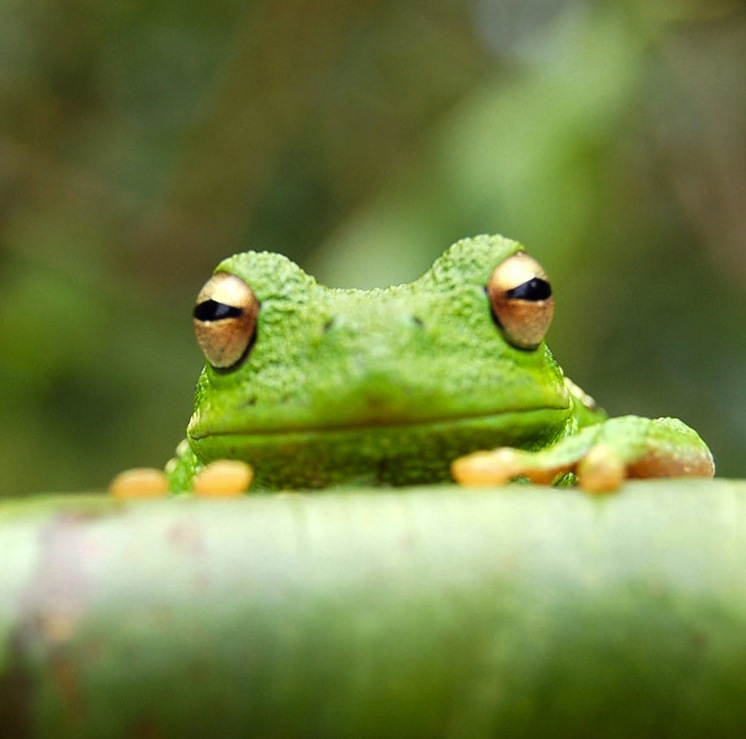
\includegraphics[width=0.5\textwidth]{frog.jpg}
% \caption{\label{fig:frog}This is a figure caption.}
% \end{figure}

% \begin{table}
% \centering
% \begin{tabular}{l|r}
% Item & Quantity \\\hline
% Widgets & 42 \\
% Gadgets & 13
% \end{tabular}
% \caption{\label{tab:widgets}An example table.}
% \end{table}

\section{Future Works}

\LaTeX{} is great at typesetting mathematics. Let $X_1, X_2, \ldots, X_n$ be a sequence of independent and identically distributed random variables with $\text{E}[X_i] = \mu$ and $\text{Var}[X_i] = \sigma^2 < \infty$, and let
$$S_n = \frac{X_1 + X_2 + \cdots + X_n}{n}
      = \frac{1}{n}\sum_{i}^{n} X_i$$
denote their mean. Then as $n$ approaches infinity, the random variables $\sqrt{n}(S_n - \mu)$ converge in distribution to a normal $\mathcal{N}(0, \sigma^2)$.

\section{Conclusion}

You can make lists with automatic numbering \dots

\begin{enumerate}
\item Like this,
\item and like this.
\end{enumerate}
\dots or bullet points \dots
\begin{itemize}
\item Like this,
\item and like this.
\end{itemize}

We hope you find write\LaTeX\ useful, and please let us know if you have any feedback using the help menu above.

\bibliographystyle{acm}
\bibliography{bib1.bib}

\end{document} to your LaTeX file where you want your
% title page.
%
%%%%%%%%%%%%%%%%%%%%%%%%%%%%%%%%%%%%%%%%%
%\title{Title page with logo}
%----------------------------------------------------------------------------------------
%	PACKAGES AND OTHER DOCUMENT CONFIGURATIONS
%----------------------------------------------------------------------------------------

\documentclass[12pt]{article}
\usepackage[english]{babel}
\usepackage[utf8x]{inputenc}
\usepackage{amsmath}
\usepackage{graphicx}
\usepackage{algorithm}
\usepackage[noend]{algpseudocode}
\usepackage[colorinlistoftodos]{todonotes}

\begin{document}

\begin{titlepage}

\newcommand{\HRule}{\rule{\linewidth}{0.5mm}} % Defines a new command for the horizontal lines, change thickness here

\center % Center everything on the page
 
%----------------------------------------------------------------------------------------
%	HEADING SECTIONS
%----------------------------------------------------------------------------------------

\textsc{\LARGE University of Texas at San Antonio}\\[1.5cm] % Name of your university/college
\textsc{\Large Department of Computer Science}\\[0.5cm] % Major heading such as course name
\textsc{\large CS-6953-012: Independent Study}\\[0.5cm] % Minor heading such as course title

%----------------------------------------------------------------------------------------
%	TITLE SECTION
%----------------------------------------------------------------------------------------

\HRule \\[0.4cm]
{ \huge \bfseries Feature Selection in TF-DNA using Correlation Analysis}\\[0.4cm] % Title of your document
\HRule \\[1.5cm]
 
%----------------------------------------------------------------------------------------
%	AUTHOR SECTION
%----------------------------------------------------------------------------------------

\begin{minipage}{0.4\textwidth}
\begin{flushleft} \large
\emph{Author:}\\
Rifatul Islam % Your name
\end{flushleft}
\end{minipage}
~
\begin{minipage}{0.4\textwidth}
\begin{flushright} \large
\emph{Supervisor:} \\
Dr. Jianhua Ruan % Supervisor's Name
\end{flushright}
\end{minipage}\\[2cm]

% If you don't want a supervisor, uncomment the two lines below and remove the section above
%\Large \emph{Author:}\\
%John \textsc{Smith}\\[3cm] % Your name

%----------------------------------------------------------------------------------------
%	LOGO SECTION
%----------------------------------------------------------------------------------------


\includegraphics{logo.jpg}\\[1cm] % Include a department/university logo - this will require the graphicx package

%----------------------------------------------------------------------------------------
%	DATE SECTION
%----------------------------------------------------------------------------------------

 {\large \today}\\[2cm] % Date, change the \today to a set date if you want to be precise

%----------------------------------------------------------------------------------------

\vfill % Fill the rest of the page with whitespace

\end{titlepage}

\begin{abstract}
Feature selection of the genes with respect to their corresponding TF is an important study in bioinformatics and generally researchers in bioinformatics want to know which conditions in genes and corresponding TF-DNA are related. In this study we investigated how can we extract the important features from the gene expression that are correlated with the corresponding TF using correlation analysis. We proposed a correlation based algorithm that selects the appropriate gene conditions based on correlation measurement and outputs the gene conditions that are highly related. 

\end{abstract}

\section{Introduction}
The protein that controls the rate of transcription of genetic information from DNA to messenger RNA by binding to a specific DNA sequence is known as the Transcription Factor(TF) which plays an important role in regulating genes \cite{wiki:tf123}. TFs work in coordination with other proteins by activating or blocking the RNA polymerase to specific genes. Transcription factors bind to either enhancer or promoter regions of DNA adjacent to the genes that they regulate. In this paper I tried to investigate which gene conditions are highly correlated with their corresponding TFs. We conduct our study based on simulated TF and Gene expression and used correlation analysis to extract the important feature from the genes. \\

We presented an algorithm that can extract the features from a given TF and their corresponding GENEs. In our study we designed a data generator that can generate the random data for the TF and the corresponding Genes. We intentionally put random data and values that are not correlated. Finally we used our algorithm to extract the correlated conditions from the random set of data. The algorithm works with an average accuracy of 90\%. 
\\ 

In the following section I will be discussing more details about our approach and results. Section 2 will include the Details of our experiments we presented the algorithm in section 2.2. In section 3 we discussed about the future direction of this study and how it can be improved further. We conclude our work by discussion the limitation of our algorithm. 


\section{Methodology}
In this section we will be discussing about the details about our approach to feature selection. To conduct our experiment we generate the TF and Gene data randomly with some data uniform random generation that generates data randomly with some intended not correlated data. Then we shuffle the data enough time so that the correlated and non-correlated data is mixed up. The goal is to figure out those conditions in the GENE data which are correlated with their corresponding Transcription Factor. The following section contains more detailed about the experiment setup, algorithm and result. 

\subsection{Experiment Setup}
We conducted our experiment in a core i7(7th Gen) with 16GB of RAM machine running on Linux based operating system(Ubuntu 18.04). We choose python version:3.6 as a programming language for convenience with the availability of data analysis packages. For data generation we use normal distribution with some intentionally added non-correlated data. For example: with 100 TF data randomly generated we generate 80 corresponding GENE values were generated that are correlated and 20 are generated that are not correlated. We use standard shuffling method to mix the correlated and non-correlated data. Then our algorithm was designed to extract the highest correlated gene value(in this case 80) that are correlated with the corresponding TF value.

\subsection{Algorithm}
In this subsection we will be discussing our algorithm in extracting the important feature of the generated TF and GENE data. Our algorithm is an iterative based algorithm which takes input as the GENE values $G$ and TF value $T$ and returns the list of correlated GENE value $G_{cor}$ and TF value $T_{cor}$. Our algorithm uses Pearson correlation analysis to select the correlated features in an iterative manner.

In this subsection we will be discussing our algorithm in extracting the important feature of the generated TF and GENE data. Our algorithm is an iterative based algorithm which takes input as the GENE values $G$ and TF value $T$ and returns the list of correlated GENE value $G_{cor}$ and TF value $T_{cor}$. Our algorithm uses Pearson correlation analysis to select the correlated features in an iterative manner.

In this subsection we will be discussing our algorithm in extracting the important feature of the generated TF and GENE data. Our algorithm is an iterative based algorithm which takes input as the GENE values $G$ and TF value $T$ and returns the list of correlated GENE value $G_{cor}$ and TF value $T_{cor}$. Our algorithm uses Pearson correlation analysis to select the correlated features in an iterative manner.


\begin{algorithm}
\caption{Iterative Feature Selection}\label{iter}
\begin{algorithmic}[1]
\Procedure{Iter correlation}{T, G, n}

\State $ GN_{corr}, TF_{corr} \gets  \textit{top\_fitted(T, G)}$
\State $ G', T'  \gets  \textit{update(T,G, TF\_{corr}, GN\_{corr})} $

\While {($\forall \, value \,\, G' \, and \, T' $)}: 
	\For {($item \, in \,G' \, and \, T'$)}:
    	\State $ GN_{corr}, TF_{corr} \gets G[item], T[item]$
        \State $corr[] \gets pearsonr(GN_{corr}, TF_{corr})$
    \EndFor
    
    \State bucket $\gets$ \( \log_2 |G'| \)
    \State $ GN_{corr} , TF_{corr} \gets  \textit{choose(T', G', bucket, corr[])}$
   \State $ G', T'  \gets  \textit{update(T,G, TF\_{corr}, GN\_{corr})} $
\EndWhile

\For {($item \,\, in \,GN_{corr} \, and \, TF_{corr}$)}:
    \State $ GN_{corr}, TF_{corr} \gets G[item], T[item]$
    \State $corr[] \gets pearsonr(GN_{corr}, TF_{corr})$
\EndFor

\EndProcedure
\end{algorithmic}
\end{algorithm}

In this subsection we will be discussing our algorithm in extracting the important feature of the generated TF and GENE data. Our algorithm is an iterative based algorithm which takes input as the GENE values $G$ and TF value $T$ and returns the list of correlated GENE value $G_{cor}$ and TF value $T_{cor}$. Our algorithm uses Pearson correlation analysis to select the correlated features in an iterative manner.


\subsection{Result}

Use the table  and tabular commands for basic tables --- see Table~\ref{tab:widgets}, for example. You can upload a figure (JPEG, PNG or PDF) using the files menu. To include it in your document, use the includegraphics command as in the code for Figure~\ref{fig:frog} below.

% Commands to include a figure:
% \begin{figure}
% \centering
% 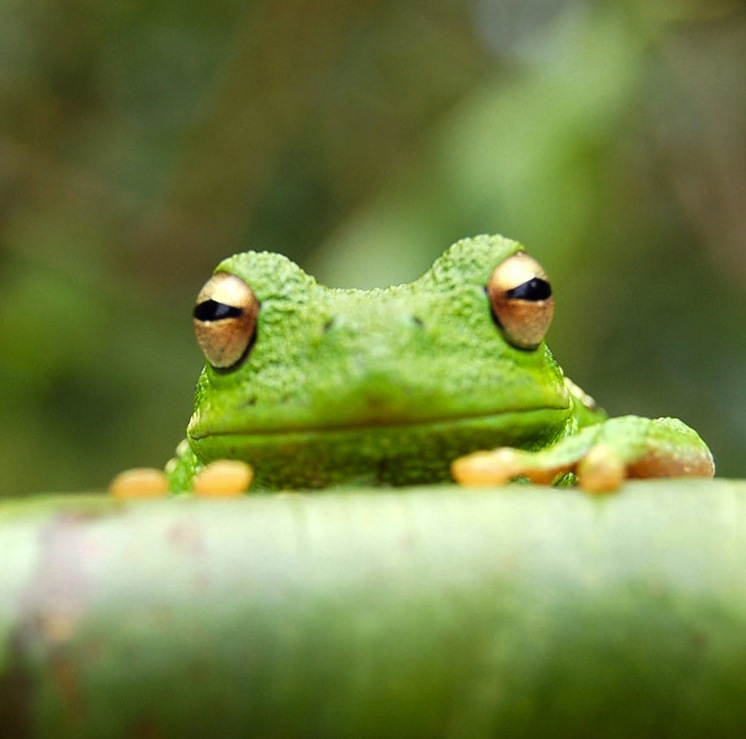
\includegraphics[width=0.5\textwidth]{frog.jpg}
% \caption{\label{fig:frog}This is a figure caption.}
% \end{figure}

% \begin{table}
% \centering
% \begin{tabular}{l|r}
% Item & Quantity \\\hline
% Widgets & 42 \\
% Gadgets & 13
% \end{tabular}
% \caption{\label{tab:widgets}An example table.}
% \end{table}

\section{Future Works}

\LaTeX{} is great at typesetting mathematics. Let $X_1, X_2, \ldots, X_n$ be a sequence of independent and identically distributed random variables with $\text{E}[X_i] = \mu$ and $\text{Var}[X_i] = \sigma^2 < \infty$, and let
$$S_n = \frac{X_1 + X_2 + \cdots + X_n}{n}
      = \frac{1}{n}\sum_{i}^{n} X_i$$
denote their mean. Then as $n$ approaches infinity, the random variables $\sqrt{n}(S_n - \mu)$ converge in distribution to a normal $\mathcal{N}(0, \sigma^2)$.

\section{Conclusion}

You can make lists with automatic numbering \dots

\begin{enumerate}
\item Like this,
\item and like this.
\end{enumerate}
\dots or bullet points \dots
\begin{itemize}
\item Like this,
\item and like this.
\end{itemize}

We hope you find write\LaTeX\ useful, and please let us know if you have any feedback using the help menu above.

\bibliographystyle{acm}
\bibliography{bib1.bib}

\end{document}